\documentclass[usenames,dvipsnames,notes]{beamer}
\usepackage{ifthen}
\usepackage{xcolor}
\usepackage{pgfplots}
\usepackage{amsmath}
\usepackage{centernot}
\usepackage{pifont}
\usepackage{tabularx}
\usepackage{makecell}
\usepackage{cuted}
\usepackage{booktabs}
\usepackage{array}
\usepackage{CJKutf8}
\usepackage{textcomp}

\usepackage{pgfpages}
%\setbeameroption{show notes on second screen}

\newcommand\w[1]{\textit{#1}}


\input ../beamer-style
\input ../std-macros
\input ../macros

\AtBeginSection[]
{
    \begin{frame}
        \frametitle{Table of Contents}
        \tableofcontents[currentsection]
    \end{frame}
}
\parskip=10pt

\title[CSCI-GA.2590]{Text Classification}
\author[He He]{He He
}
\institute[NYU]{New York University}
\date{\today}

\begin{document}

\begin{frame}
\titlepage
\end{frame}

\begin{frame}
    {Text classification}
    \begin{itemize}
        \item Application
            \begin{itemize}
                \item Spam filter, sentiment classification, document classification, ...
                \item Textual entailment, paraphrase detection, ...
            \end{itemize}
    \end{itemize}
    \vspace{7em}
\end{frame}

\section{Generative models: naive Bayes}

\begin{frame}
    {Intuition}
    \begin{itemize}
        \itemsep1em
        \item[]Example: sentiment classification for movie reviews
    \begin{itemize}
        \item[] \textit{Bromwell High is a cartoon comedy. It ran at the same time as some other programs about school life, such as "Teachers". My 35 years in the teaching profession lead me to believe that Bromwell High's satire is much closer to reality than is "Teachers". The scramble to survive financially, the insightful students who can see right through their pathetic teachers' pomp, the pettiness of the whole situation, all remind me of the schools I knew and their students...}

        \item[] Label: positive 
    \end{itemize}
    \pause
\item[]\emph{Idea}: assign a score of positivity/negativity for each word

\item[][demo]
    \end{itemize}
\end{frame}

\begin{frame}
    {Side note: tokenization}
    Splitting a string of text $s$ to a sequence of \textbf{tokens} $[x_1, \ldots x_n]$.

    \emph{Language-specific solutions}\\
    \begin{itemize}
        \itemsep1em
        \item Regular expression: ``I didn't watch the movie''. $\rightarrow$ [``I'', ``did'', ``n't'', ``watch'', ``the'', ``movie'', ``.''] 
        \item Dictionary / sequence labeler: 
            \begin{CJK*}{UTF8}{gbsn}
                ``我没有去看电影。'' $\rightarrow$ [``我'', ``没有'', ``去'', ``看'', ``电影'', ``。'']
            \end{CJK*}
    \end{itemize}

    \pause
    \emph{General solution}: don't split by words\\
    \begin{itemize}
        \item Characters:
            [``u'', ``n'', ``a'', ``f'', ``f'', ``a'', ``b'', ``l'', ``e'']
        \item Subword (e.g. byte pair encoding):
            [``un'', ``aff'', ``able\#'']
    \end{itemize}
\end{frame}

\begin{frame}
    {Problem formulation}
    \begin{itemize}
        \itemsep1em
        \item \emph{Input}: a sequence of tokens $X=(X_1, \ldots X_n)$ where $X_i \in \mathcal{V}$.
        \item \emph{Output}: label $Y\in \pc{0, 1}$.
        \item \emph{Probabilistic model}:
            $$
            f(x) = \begin{cases}
 1 & \text{if $p_\theta(y\mid x) > 0.5$} \\
 0 & \text{otherwise}
 \end{cases} ,
            $$
            where $p_\theta$ is a distribution parametrized by $\theta\in{\Theta}$.
        \item Question: how to choose $p_\theta$? (\textbf{inductive bias})
    \end{itemize}
\end{frame}

\begin{frame}
    {Model $p(y\mid x)$}
    How to write a review:\\
    \begin{enumerate}
        \item Decide the sentiment by flipping a coin
        \item Generate word sequentially conditioned on the sentiment 
    \end{enumerate}
    \begin{block}
        {Bayes rule}
        $$
        p(y\mid x) = \frac{p(x\mid y)p(y)}{p(x)}
        = \frac{p(x\mid y)p(y)}{\sum_{y\in\mathcal{Y}} p(x\mid y)p(y)}
        $$
    \end{block}
    \begin{itemize}
        \item $p(y)$
        \item $p(x\mid y)$
    \end{itemize}
\end{frame}

\begin{frame}
    {Naive Bayes models}
    \begin{block}
    {Naive Bayes assumption}
        The input features are \textbf{conditionally independent} given the label:
        $$
        p(x\mid y) = \prod_{i=1}^n p(x_i\mid y) \;.
        $$
    \end{block}
    A strong assumption, but works surprisingly well in practice.

    Note: $p(x_i\mid y)$ doesn't have to be a categorical distribution.

    \emph{Inference}:\\
    \vspace{5em}
\end{frame}

\begin{frame}
    {Maximum likelihood estimation}
    \emph{Task}: estimate parameters $\theta$ of a distribution $p(y; \theta)$ given i.i.d. samples $D=\p{y_1, \ldots, y_N}$ from the distribution.

    \emph{Goal}: find the parameters that make the observed data most probable.

    \textbf{Likelihood function} of $\theta$ given $D$:
    $$
    L(\theta; D) \eqdef p(D;\theta) = \prod_{i=1}^N p(y_i; \theta) \;.
    $$

    \textbf{Maximum likelihood estimator}:\\
    \vspace{7em}
\end{frame}

\begin{frame}
    {MLE and ERM}
\end{frame}

\begin{frame}
    {MLE for our Naive Bayes model}
\end{frame}

\begin{frame}
    {MLE for our Naive Bayes model}
    MLE solution:
    \begin{align*}
        \text{count}(w, y) &\eqdef \text{frequency of $w$ in documents with label $y$}\\ 
        p(w\mid y) &= \frac{\text{count}(w, y)}{\sum_{w\in\mathcal{V}}\text{count}(w, y)}\\
        p(y=k) &= \frac{\sum_{i=1}^N \1\p{y^{(i)}=k}}{N}
    \end{align*}
    \pause
    \textbf{Smoothing}: reserve probability mass for unseen words
    $$
        p(w\mid y) = \frac{{\color{blue}\alpha} + \text{count}(w, y)}{\sum_{w\in\mathcal{V}}\text{count}(w, y) + {\color{blue}\alpha|\mathcal{V}|}}
    $$
    Laplace smoothing: $\alpha=1$
\end{frame}

\begin{frame}
    {Feature design}
        Naive Bayes doesn't have to use single words as features
    \begin{itemize}
        \itemsep1em
        \item Lexicons, e.g. LIWC.
        \item Task-specific features, e.g. is the subject all caps.
        \item Bytes and characters, e.g. used in language ID detection.
    \end{itemize}
\end{frame}

\section{Discriminative models: logistic regression}

\begin{frame}
    {Discriminative models}
    \emph{Key idea}: directly model the conditional distribution $p(y\mid x)$
    \begin{table}
        \renewcommand{\arraystretch}{1.5}
        \begin{tabular}{cc}
            generative models & discriminative models \\
            \hline
            $p(x,y)$ & $p(y\mid x)$ \\
            more assumption & - \\
            generative story & feature extractor
        \end{tabular}
    \end{table}
\end{frame}

\begin{frame}
    {Model $p(y\mid x)$}
    How to model $p(y\mid x)$?
    \begin{itemize}
        \item[] Bernoulli:
        \item[] Bring in $x$:
    \end{itemize}

    Linear predictor:\\
    \vspace{7em}
\end{frame}

\begin{frame}
    {Logistic regression}
    Map $w\cdot\phi(x) \in\mathbb{R}$ to a probability by the \textbf{logistic function}
    \begin{center}
        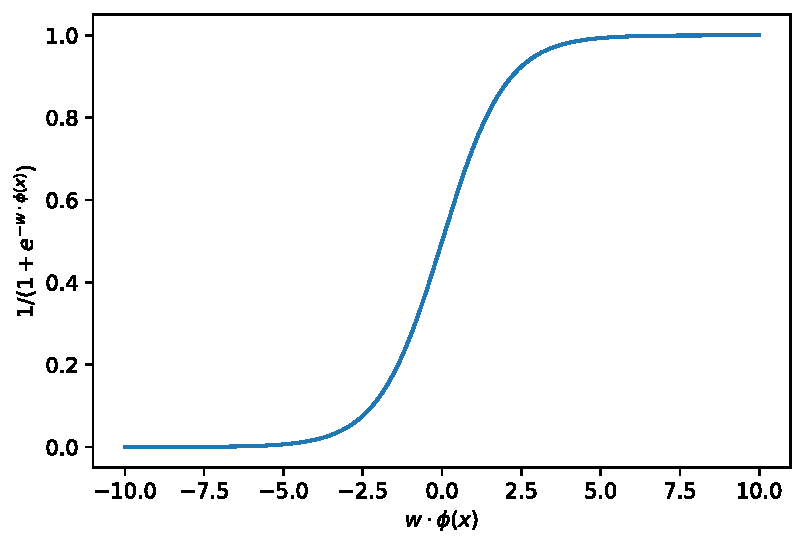
\includegraphics[height=3cm]{figures/logistic}
    \end{center}
    \begin{align*}
    p(y=1\mid x; w) &= \frac{1}{1 + e^{-w\cdot\phi(x)}} \quad (y\in \pc{0,1})\\
        p(y=k\mid x; w) &= \frac{e^{w_k\cdot\phi(x)}}{\sum_{i\in\mathcal{Y}}e^{w_i\cdot\phi(x)}} \quad (y\in \pc{1, \ldots, K}) && \text{soft argmax}
    \end{align*}
\end{frame}

\begin{frame}
    {MLE for logistic regression}
\end{frame}

\begin{frame}
    {BoW representation}
    \textbf{Feature extractor}: $\phi\colon \mathcal{V}^n \rightarrow \mathbb{R}^d$.

    \emph{Idea}: a sentence is the ``sum'' of words.

    Example:
    \begin{align*}
        \mathcal{V} &= \pc{\w{the}, \w{a}, \w{an}, \w{in}, \w{for}, \w{penny}, \w{pound}}\\
        \text{sentence} &= \w{in for a penny, in for a pound} \\
        x &= \p{\w{in}, \w{for}, \w{a}, \w{penny}, \w{in}, \w{for}, \w{a}, \w{pound}}
    \end{align*}
    \vspace{7em}
\end{frame}

\begin{frame}
    {Compare with naive Bayes}
    \begin{itemize}
        \itemsep2em
        \item Our naive Bayes model ($x_i \in \pc{1, \ldots, |\sV|}$):
            $$
            X_i \mid Y=y \sim \text{Categorical}(\theta_{1,y}, \ldots, \theta_{|\sV|, y}) \;.
            $$
        \item The naive Bayes generative story corresponds to a multinomial distribution of the BoW count vector:
            $$
            \phi_{\text{BoW}}(X) \mid Y=y \sim \text{Multinomial}(\theta_{1,y}, \ldots, \theta_{|\sV|,y}, n) \;.
            $$
        \item Both multinomial naive Bayes and logistic regression learn a linear separator $w\cdot\phi_{\text{BoW}}(x)+b=0$.
    \end{itemize}
    Question: what's the advantage of using logistic regression?
\end{frame}

\begin{frame}
    {Feature extractor}
    Define each feature as a function $\phi_i\colon \mathcal{X} \rightarrow \BR$.
    \begin{align*}
 \phi_1(x) &= \begin{cases}
 1 & \text{$x$ contains ``happy''} \\
 0 & \text{otherwise}
 \end{cases} ,
 \\
 \phi_2(x) &= \begin{cases}
 1 & \text{$x$ contains words with suffix ``yyyy''} \\
 0 & \text{otherwise}
 \end{cases} .
    \end{align*}
    In practice, use a dictionary
    $$
    \texttt{feature\_vector}[\texttt{"prefix=un+suffix=ing"}] = 1
    $$
\end{frame}

\begin{frame}
    {Feature vectors for multiclass classification}
    Multinomial logistic regression
    \begin{tikzpicture}
        \node (a) {
            \begin{minipage}{\textwidth}
            \begin{align*}
        p(y=k\mid x; w) =
             \frac{e^{{\color{blue}w_k\cdot\phi(x)}}}
                {\sum_{i\in\mathcal{Y}}e^{w_i\cdot\phi(x)}} \quad (y\in \pc{1, \ldots, K})
            \end{align*}
            \end{minipage}
};
        \node(b) [below= of a] {
            \begin{minipage}{\textwidth}
    $$
        p(y=k\mid x; w) =
                \frac{e^{{\color{blue}w\cdot\Psi(x, k)}}}{\sum_{i\in\mathcal{Y}}e^{w\cdot\Psi(x, i)}} \quad (y\in \pc{1, \ldots, K})
    $$
            \end{minipage}
};
        \draw[arrow] (a) -- (b);
    \end{tikzpicture}
    Multivector construction of $\Psi(x,y)$:
    \vspace{6em}
\end{frame}

\begin{frame}
    {N-gram features}
    Potential problems with the the BoW representation?
    \vspace{3em}

    \pause
    \textbf{N-gram} features:
    \begin{center}
        \textit{in for a penny , in for a pound}
    \end{center}
    \begin{itemize}
        \item Unigram
        \item Bigram
        \item Trigram
    \end{itemize}

    What's the pros/cons of using higher order n-grams?
\end{frame}

\section{Regularization, model selection, evaluation}

\begin{frame}
    {Bias-variance trade-off}
    Error decomposition:
    \begin{align*}
        \text{risk}(h) - \text{risk}(h^*) = \text{approximation error} + \text{estimation error}
    \end{align*}
    \vspace{5em}

    Larger hypothesis class: approximation error $\downarrow$, estimation error $\uparrow$

    Smaller hypothesis class: approximation error $\uparrow$, estimation error $\downarrow$

    How to control the size of the hypothesis class?
\end{frame}

\begin{frame}
    {Reduce the dimensionality}
    Linear predictors: $\sH = \pc{w : w \in \BR^d}$

    Reduce the number of features:\\
    \vspace{7em}

    \pause
    Other predictors:\\
    \begin{itemize}
        \item Depth of decision trees
        \item Degree of polynomials
        \item Number of decision stumps in boosting
    \end{itemize}
\end{frame}

\begin{frame}
    {Regularization}
    Reduce the norm of $w$:
    $$
    \min_w \underbrace{\frac{1}{N}\sum_{i=1}^N L(x^{(i)}, y^{(i)}, w)}_{\text{average loss}}
    + \underbrace{\frac{\lambda}{2}\|w\|_2^2}_{\ell_2 \text{ norm}}
    $$

    Why is small norm good? Small change in the input doesn't cause large change in the output.
    \vspace{7em}
\end{frame}

\begin{frame}
    {Gradient descent with $\ell_2$ regularization}
    Run SGD on 
    $$
    \min_w \underbrace{\frac{1}{N}\sum_{i=1}^N L(x^{(i)}, y^{(i)}, w)}_{\text{average loss}}
    + \underbrace{\frac{\lambda}{2}\|w\|_2^2}_{\ell_2 \text{ norm}}
    $$

    Also called \textbf{weight decay} in the deep learning literature:
    $$
    w \leftarrow w - \eta(\nabla_w L(x, y, w) + {\color{blue}\lambda w})
    $$

    Shrink $w$ in each update.
\end{frame}

\begin{frame}
    {Hyperparameter tuning}
    \textbf{Hyperparameters}: parameters of the learning algorithm (not the model)

    Example: use MLE to learn a logistic regression model using BoW features \\
    \vspace{7em} 

    \pause
    How do we select hyperparameters?\\
    \begin{itemize}
        \item[] Pick those minimizing the training error 
        \item[] Pick those minimizing the test error 
    \end{itemize}
\end{frame}

\begin{frame}
    {Validation}
    \textbf{Validation set}: a subset of the training data reserved for tuning the learning algorithm (also called the \textbf{development set}).

    \textbf{$K$-fold cross validation}\\
    \vspace{10em}

    It's important to look at the data and errors during development, but \textcolor{red}{not the test set}.
\end{frame}

\begin{frame}
    {Evaluation}
    \begin{itemize}
        \itemsep3em
        \item Accuracy
        \item Precision
        \item Recall 
        \item F1
        \item Macro vs micro average
    \end{itemize}
\end{frame}

\end{document}
